\section{JavaScript}
\label{js}

JavaScript ist eine Programmiersprache/Skriptsprache, die üblicherweise in Webseiten Verwendung findet. Sie wird jedoch auch noch vielen Umgebungen außerhalb der Website Entwicklung benutzt, 
wie zum Beispiel \nameref{nodejs}.
JavaScript besitzt First-Class-Funktions (Funktion erster Klasse). Außerdem is JS eine prototypbasierte Sprache, welche mehreren Paradigmen folgt, dynamisch ist und 
objektorientiert ist. JavaScript ist plattformunabhängig. Zusätzlich ist es sehr kompakt und ressourcenschonend. 
JavaScript sollte man nicht mit Java verwechseln. Sie sind beide Handelsmarken. Sie besitzen beide eine unterschiedliche Syntax, Semantik und Verwendung.~\cite{JS}

\subsection{First-Class-Funktions}
Funktionen erster Klasse werden wie Variablen behandelt. Bei einer Programmiersprache welche First-Class-Funktionen besitzt, kann man Funktionen als Parameter übergeben, einer Variable zuweisen oder
einer anderen Funktion zurückgegeben werden.
\pagebreak

\begin{center}
    \subsubsection{Beispiel für die Zuweisung einer Funktion an eine Variable}
\begin{figure}[htbp]
    \centerline{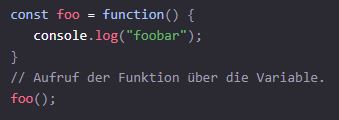
\includegraphics{Theorie/JavaScript/Funktion-in-Variable.png}}
    \caption{Zuweisung einer Funktion an eine Variable.~\cite{First-Class-Funktion}}
\end{figure}
\end{center}
Hier wird der Variable \textit{foo} eine anonyme Funktion zugewiesen, welche und in der Konsole eine Ausgaben liefert.
Diese Funktion wird dann ganz einfach über die Variable mittels den zwei Klammern aufgerufen.


\begin{center}
    \subsubsection{Beispiel für das Übergeben einer Funktion als Argument}
\begin{figure}[htbp]
    \centerline{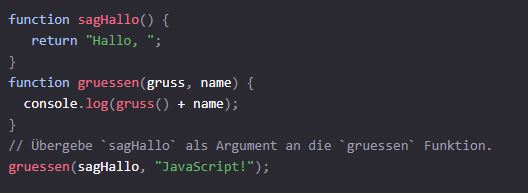
\includegraphics{Theorie/JavaScript/Funktion-als-Argument.png}}
    \caption{Übergeben einer Funktion als Argument.~\cite{First-Class-Funktion}}
\end{figure}
\end{center}
Hier übergeben wird er Funktion \textit{gruessen} 2 Parameter. Als einer dieser beiden Parameter übergeben wir die Funktion \textit{sagHallo} welche ``Hallo, `` als return liefert.
Führen wir nun die Methode gruessen mit diesen Parametern aus, wird in die Console der Satz \textit{``Hallo, Javascript``} geschrieben.
\pagebreak

\begin{center}
    \subsubsection{Eine Funktion als Return}
\begin{figure}[htbp]
    \centerline{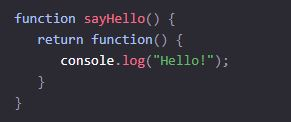
\includegraphics{Theorie/JavaScript/Funktion-als-Return.png}}
    \caption{Funktion als Return.~\cite{First-Class-Funktion}}
\end{figure}
\end{center}
Hier wird ganz einfach als return Wert eine Funktion übergeben.

\subsection{Objektorientierte Programmierung}
Objektorientierte Programmierung (OOP) eignet sich gut für große und komplexe Software, die aktiv aktualisiert oder gewartet werden muss. OOP konzentriert sich nicht auf die Logik, 
sondern auf die Objekte, mit denen das Programm interagieren soll. Der Aufbau für das Programm bei der Objektorientierten Entwicklung ist auch für das Entwickeln von Vorteil.
Andere Vorteile von OOP sind die Wiederverwendbarkeit von Code, Skalierbarkeit und die Effizienz.~\cite{OOP}

\subsubsection{Prinzipien von OOP}
\begin{description}
\item[Verkapselung]\hfill \\
 Objekte werden privat innerhalb einer definierten Grenze oder Klasse gehalten implementiert und andere Objekte haben keinen Zugriff auf diese Klasse und keine Berechtigung
 Änderungen vorzunehmen. Dies versichert eine größere Programmiersicherheit
\item[Abstraktion]\hfill \\
Objekte verbergen den unnötigen Implementierungscode und offenbaren nur interne Mechanismen, welche für andere Objekte relevant sind. Hilfreich für Entwickler um Änderungen 
und Ergänzungen vorzunehmen.
\item[Inheritance]\hfill \\
Man kann Beziehungen und Unterklassen zwischen Objekten zuweisen, um gemeinsame Logik wiederverwenden zu können. Vorteile hiervon sind eine verkürzte Entwicklungszeit und 
es sorgt für eine höhere Genauigkeit.
\end{description}

\subsubsection{Prototypbasierte Programmierung}
Ist eine andere Art von objektorientierte Programmierung bei der keine Klassen verwendet werden. Stattdessen erzeugt man Objekte durch das Kopieren von bereits existierenden 
Objekten (Prototypen). Beim Kopieren werden alle Eigenschaften des kopierten Objekts übernommen. Man kann diese auch verändern und/oder ergänzen.